		%%%%%%%%%%%%%%%%%%%%%%%%%%%%%%%%%%%%%%%%%
		% Beamer Presentation
		% LaTeX Template
		% Version 1.0 (10/11/12)
		%
		% This template has been downloaded from:
		% http://www.LaTeXTemplates.com
		%
		% License:
		% CC BY-NC-SA 3.0 (http://creativecommons.org/licenses/by-nc-sa/3.0/)
		%
		%%%%%%%%%%%%%%%%%%%%%%%%%%%%%%%%%%%%%%%%%
		
		%----------------------------------------------------------------------------------------
		%	PACKAGES AND THEMES
		%----------------------------------------------------------------------------------------
		
		\documentclass[professionalfont,fleqn]{beamer}
		% \documentclass[9pt, handout]{beamer} ## Esto es para armar una versión compacta para circular
		\setbeamercovered{transparent}
		\setlength{\mathindent}{0pt}
		
		\mode<presentation> {
		
		% The Beamer class comes with a number of default slide themes
		% which change the colors and layouts of slides. Below this is a list
		% of all the themes, uncomment each in turn to see what they look like.
		
		
		%\usetheme{default}
		%\usetheme{AnnArbor}
		%\usetheme{Antibes}
		%\usetheme{Bergen}
		%\usetheme{Berkeley}
		%\usetheme{Berlin}
		%\usetheme{Boadilla}
		%%\usetheme{CambridgeUS}
		%\usetheme{Copenhagen}
		%\usetheme{Darmstadt}
		%\usetheme{Dresden}
		%\usetheme{Frankfurt}
		%%\usetheme{Goettingen}
		%%\usetheme{Hannover}
		%\usetheme{Ilmenau}
		%\usetheme{JuanLesPins}
		\usetheme{Luebeck}
		%\usetheme{Madrid}
		%%\usetheme{Malmoe}
		%\usetheme{Marburg}
		%%\usetheme{Montpellier}
		%\usetheme{PaloAlto}
		%%\usetheme{Pittsburgh}
		%\usetheme{Rochester}
		%\usetheme{Singapore}
		%\usetheme{Szeged}
		%\usetheme{Warsaw}
		
		% As well as themes, the Beamer class has a number of color themes
		% for any slide theme. Uncomment each of these in turn to see how it
		% changes the colors of your current slide theme.
		
		%\usecolortheme{albatross}
		%%\usecolortheme{beaver}
		%\usecolortheme{beetle}
		%\usecolortheme{crane}
		%\usecolortheme{dolphin}
		%%\usecolortheme{dove}
		%\usecolortheme{fly}
		%\usecolortheme{lily}
		%\usecolortheme{orchid}
		%\usecolortheme{rose}
		%\usecolortheme{seagull}
		\usecolortheme{seahorse}
		%\usecolortheme{whale}
		%\usecolortheme{wolverine}
		
		%\setbeamertemplate{footline} % To remove the footer line in all slides uncomment this line
		%\setbeamertemplate{footline}[page number] % To replace the footer line in all slides with a simple slide count uncomment this line
		
		%\setbeamertemplate{navigation symbols}{} % To remove the navigation symbols from the bottom of all slides uncomment this line
		}
		\usepackage{amssymb}
		\usepackage{amsmath}
		
		\usepackage{graphicx}
		\graphicspath{ {Graficos/} }
		\usepackage{subfigure}
		\usepackage{booktabs} % Allows the use of \toprule, \midrule and \bottomrule in tables
		
		\newcommand*{\boxedcolor}{red}
		\makeatletter
		\renewcommand{\boxed}[1]{\textcolor{\boxedcolor}{%
				\fbox{\normalcolor\m@th$\displaystyle#1$}}}
		\makeatother
		
		%----------------------------------------------------------------------------------------
		%	TITLE PAGE
		%----------------------------------------------------------------------------------------
		
		\title[Word Trade Network]{Description of international trade using a complex network model} % The short title appears at the bottom of every slide, the full title is only on the title page
		
		\author{Diego Kozlowski} % Your name
		\institute[University of Buenos Aires] % Your institution as it will appear on the bottom of every slide, may be shorthand to save space
		{
		University of Buenos Aires\\ % Your institution for the title page
		\medskip
		\textit{diegokoz92@gmail.com} % Your email address
		}
		\date{July 21, 2018} % Date, can be changed to a custom date
		
		\begin{document}
		
		\begin{frame}
		\titlepage % Print the title page as the first slide
		\end{frame}
		
		
		\begin{frame}
		\frametitle{Introduction}
		\begin{itemize}
			\item World Trade Network as a graph
			\item Methodological decisions involve in this representation
			\item Expressions of the New International Division of labor by node centralities and clustering. 
		\end{itemize}
		
		\end{frame}
		
		\begin{frame}
		\frametitle{Overview} % Table of contents slide, comment this block out to remove it
		\tableofcontents % Throughout your presentation, if you choose to use \section{} and \subsection{} commands, these will automatically be printed on this slide as an overview of your presentation
		\end{frame}
		
		%----------------------------------------------------------------------------------------
		%	PRESENTATION SLIDES
		%----------------------------------------------------------------------------------------
		
		%------------------------------------------------
		\section{Methodology} % Sections can be created in order to organize your presentation into discrete blocks, all sections and subsections are automatically printed in the table of contents as an overview of the talk
		%------------------------------------------------
	
	
		
		\begin{frame}
		\frametitle{Data}
		Bilateral aggregated data of trade between countries, by year.
		
		\vspace*{10px}
		
		\textit{sources:}  
		\begin{itemize}
			\item {Gleditsch 1950-2000}\footnote{\url{http://privatewww.essex.ac.uk/~ksg/exptradegdp.html}}
			\item {WTO. 1997-2011}\footnote{\url{https://comtrade.un.org/}}
		\end{itemize}
		
		\end{frame}
		
		%\subsection{Construction of the network} % A subsection can be created just before a set of slides with a common theme to further break down your presentation into chunks
		\begin{frame}
		\frametitle{Bilateral trade}
		
		\begin{columns}[t]
			\column{.5\textwidth}
			
				\begin{equation*}
				a_{ij} = 
				\begin{cases} 
				1 & if \frac{x_{ij}}{x_{i\cdot}}\geq u \\
				0 & else 
				\end{cases}
				$$
				\end{equation*}
				$x_{ij}$: Total trade between countries i-j \par
				$x_{i\cdot}$: Total trade of country i
			
			\column{.5\textwidth}
			
			\begin{itemize}
				\item Two countries are connected if there is \textit{enough} trade between them.
				\item This can be either exports or imports.
				\item The graph is directed, so $a_{ij} \neq a_{ji}$.
			\end{itemize}
			
		\end{columns}
		
		\end{frame}
		
				
		
\begin{frame}
\frametitle{Producers \& Consumers}	
	\begin{columns}
		\column{.5\textwidth}
			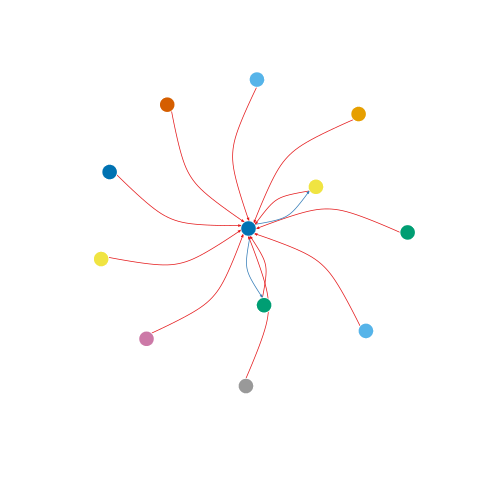
\includegraphics[width=\linewidth]{toy_graph1}
		
		\column{.65\textwidth}
		\begin{itemize}
			\item From the point of view of a country, there can not be many relevant countries. It can not have many \textbf{out edges}
			\item But they may be relevant from the point of view of other countries. They can have many \textbf{in edges} 
			\item Therefore, with the \textbf{export} data, the central nodes will be \textbf{relevant as consumers}
			\item With \textbf{import} data, central nodes will be \textbf{relevant as producers}
			
		\end{itemize}	
	\end{columns}	
\end{frame}
		
\begin{frame}
\frametitle{Producers \& Consumers}	
\begin{columns}
	\column{.5\textwidth}
	\hspace*{-0.2\linewidth}
	\includegraphics<1>[width=1.5\linewidth]{grafo_2011_1_pcnt}
	%\hspace*{-0.2\linewidth}
	\includegraphics<2>[width=1.5\linewidth]{grafo_2011_20_pcnt}
	
	\column{.5\textwidth}
	\begin{itemize}
		\item<1-> With the real data.
		\item<1> At a 1\% threshold, this phenomenon is not visually clear. 
		\item<2-> At a 20\% threshold, we can see some important nodes with lots of \textbf{in edges}
	\end{itemize}	
\end{columns}	
\end{frame}
	%------------------------------------------------
		
		\section{Results}
	
		\begin{frame}
	\frametitle{Graph representation}
	
	
		\begin{onlyenv}<1>
			%Threshold: 1\%
			\begin{center}
			\includegraphics<1>[width=.75\textwidth,height=.75\textwidth]{grafo_Circ_2011_1_pcnt}
			\end{center}
		\end{onlyenv}
	
				
	\begin{columns}[t]
		\column{.5\textwidth}
		\centering
		\includegraphics<2->[width=.7\linewidth,height=.7\linewidth]{grafo_Circ_2011_1_pcnt}\\
		%\only<2->{\texttt{1\%}}
		\includegraphics<2->[width=.7\linewidth,height=.7\linewidth]{grafoCirc_2011_5_pcnt}
		%\only<2->{\texttt{5\%}}
		\column{.5\textwidth}
		\centering
		\includegraphics<3->[width=.7\linewidth,height=.7\linewidth]{grafoCirc_2011_10_pcnt}\\
		%\only<3->{\texttt{10\%}}
		\includegraphics<4->[width=.7\linewidth,height=.7\linewidth]{grafoCirc_2011_15_pcnt}
		%\only<4->{\texttt{15\%}}
	\end{columns}
	
	\end{frame}
	
		
	\begin{frame}
		\frametitle{Exports and Imports correlation I}
		
		
		\textbf{Degree Centrality} in the graph of imports respect to the graph of exports
		\begin{columns}[c] % The "c" option specifies centered vertical alignment while the "t" option is used for top vertical alignment
	%			
		\column{.6\textwidth} % Right column and width
		\begin{flushleft}
			\begin{figure}
				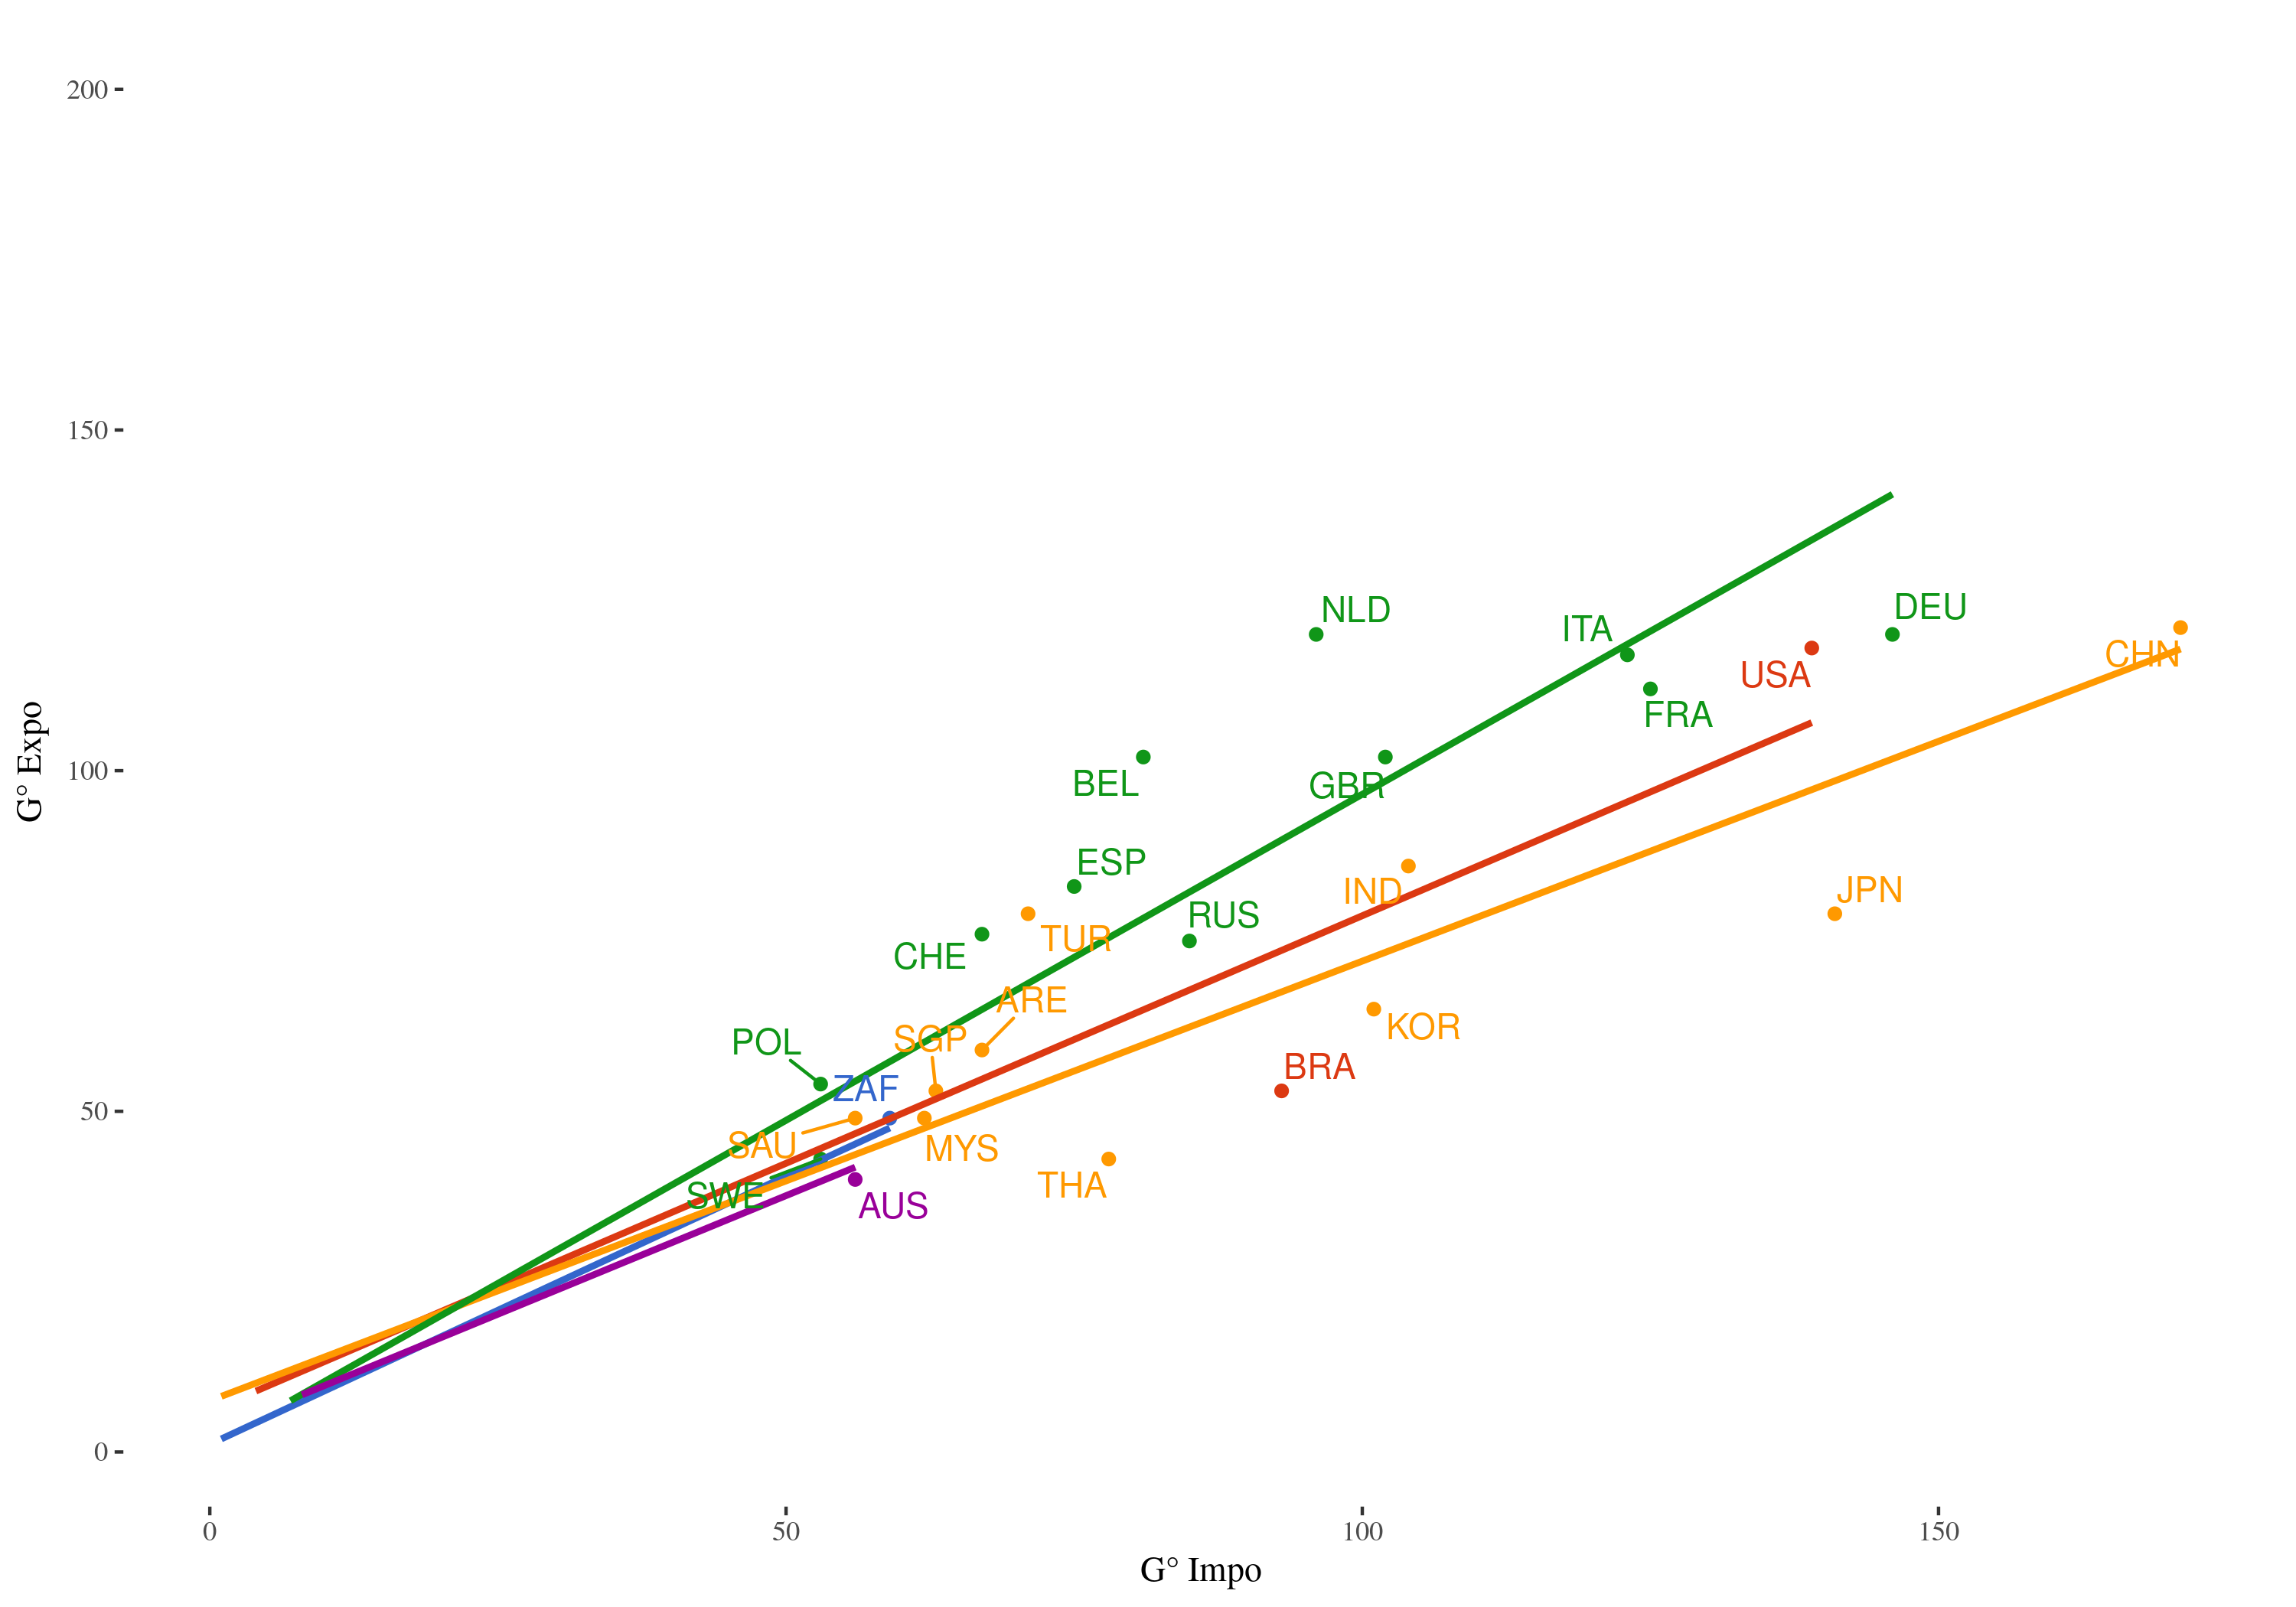
\includegraphics[width=\linewidth]{corr_grados_2011_1_pcnt}
			\end{figure}
		\end{flushleft}
		
		
		\column{.45\textwidth} % Left column and width
		\begin{itemize}
			\item 1\% Threshold: Weak dependency network.
			\item Europe has bigger role as a consumer.
			\item Asia has more centrality as a producer.
		\end{itemize}
		\end{columns}
	\end{frame}
	%%%%%	
			\begin{frame}
		\frametitle{Exports and Imports correlation II}
		\begin{columns}[c] % The "c" option specifies centered vertical alignment while the "t" option is used for top vertical alignment
			
		
		\column{.65\textwidth} % Right column and width
		\begin{flushleft}
			\begin{figure}
				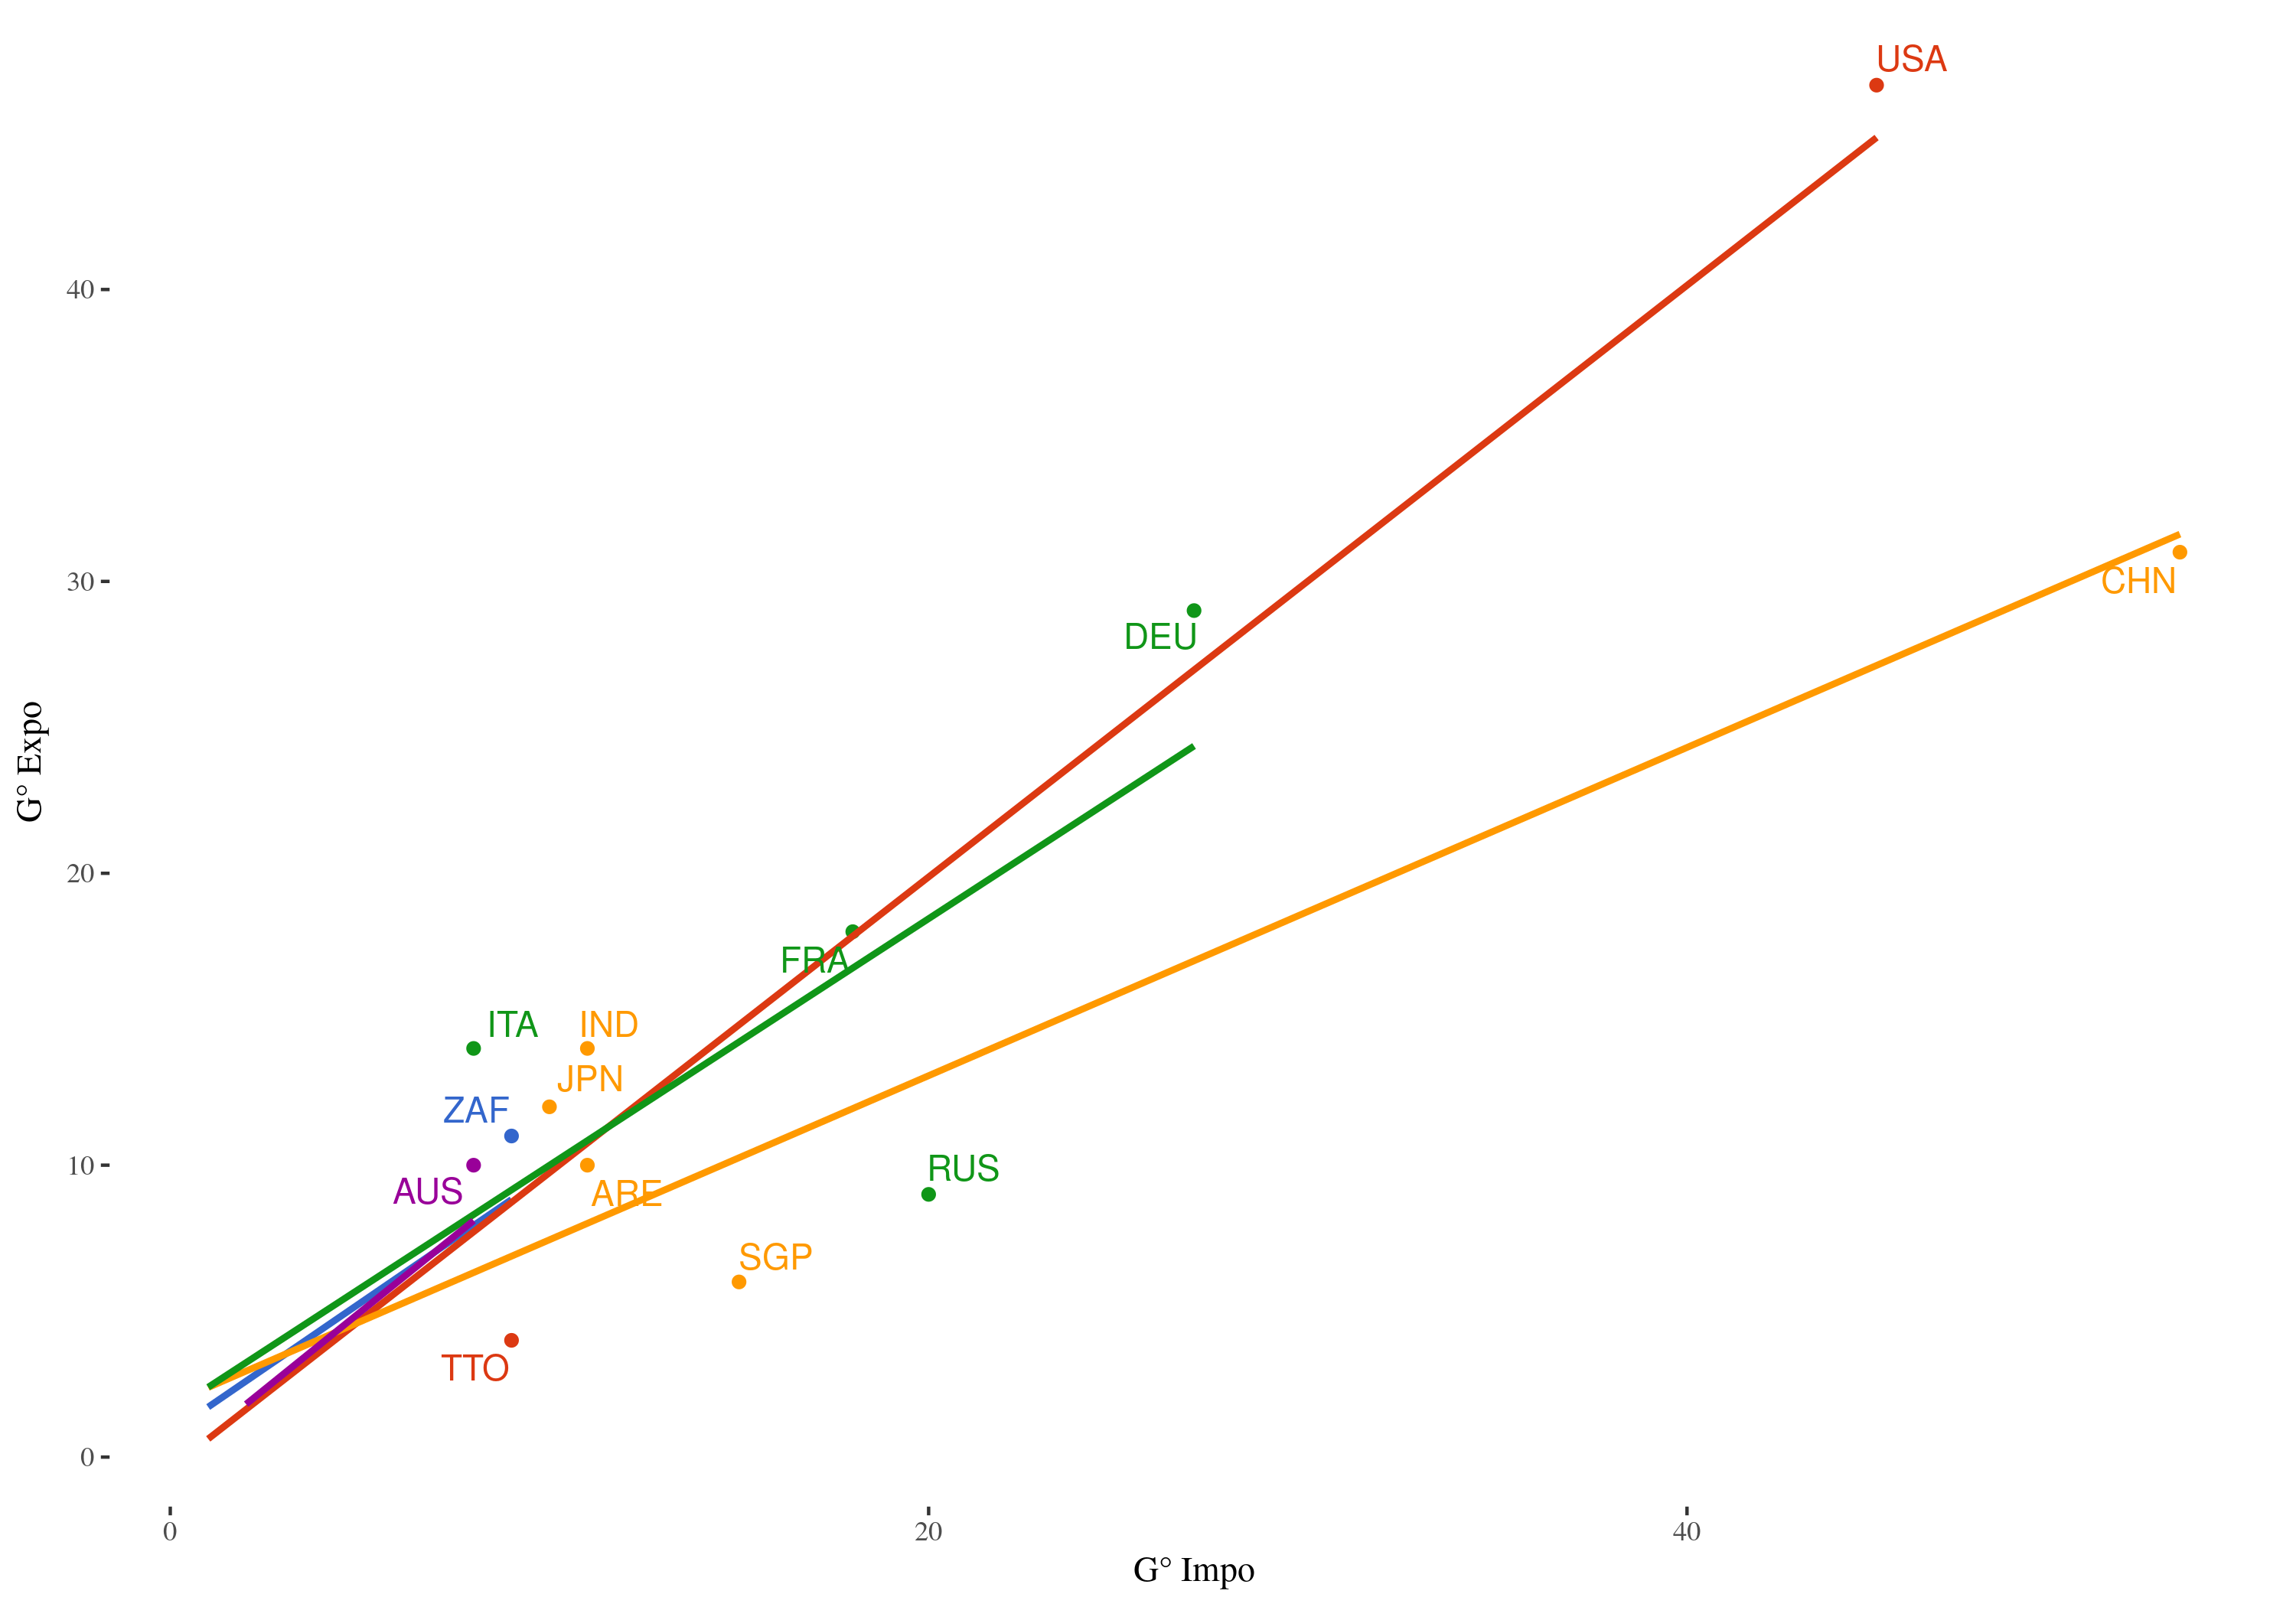
\includegraphics[width=\linewidth]{corr_grados_2011_10_pcnt}
			\end{figure}
		\end{flushleft}
		
		
		\column{.45\textwidth} % Left column and width
		\begin{itemize}
			\item 10\% Threshold
			\item USA and Germany begin to separate from the rest of the nodes, with more importance as consumers.
			\item China does also, but as a producer.
		\end{itemize}
		\end{columns}
	\end{frame}
		\begin{frame}
		
	\frametitle{Exports and Imports correlation III}
		\begin{columns}[c] % The "c" option specifies centered vertical alignment while the "t" option is used for top vertical alignment
		
	
	
	\column{.65\textwidth} % Right column and width
	\begin{flushleft}
		\begin{figure}
			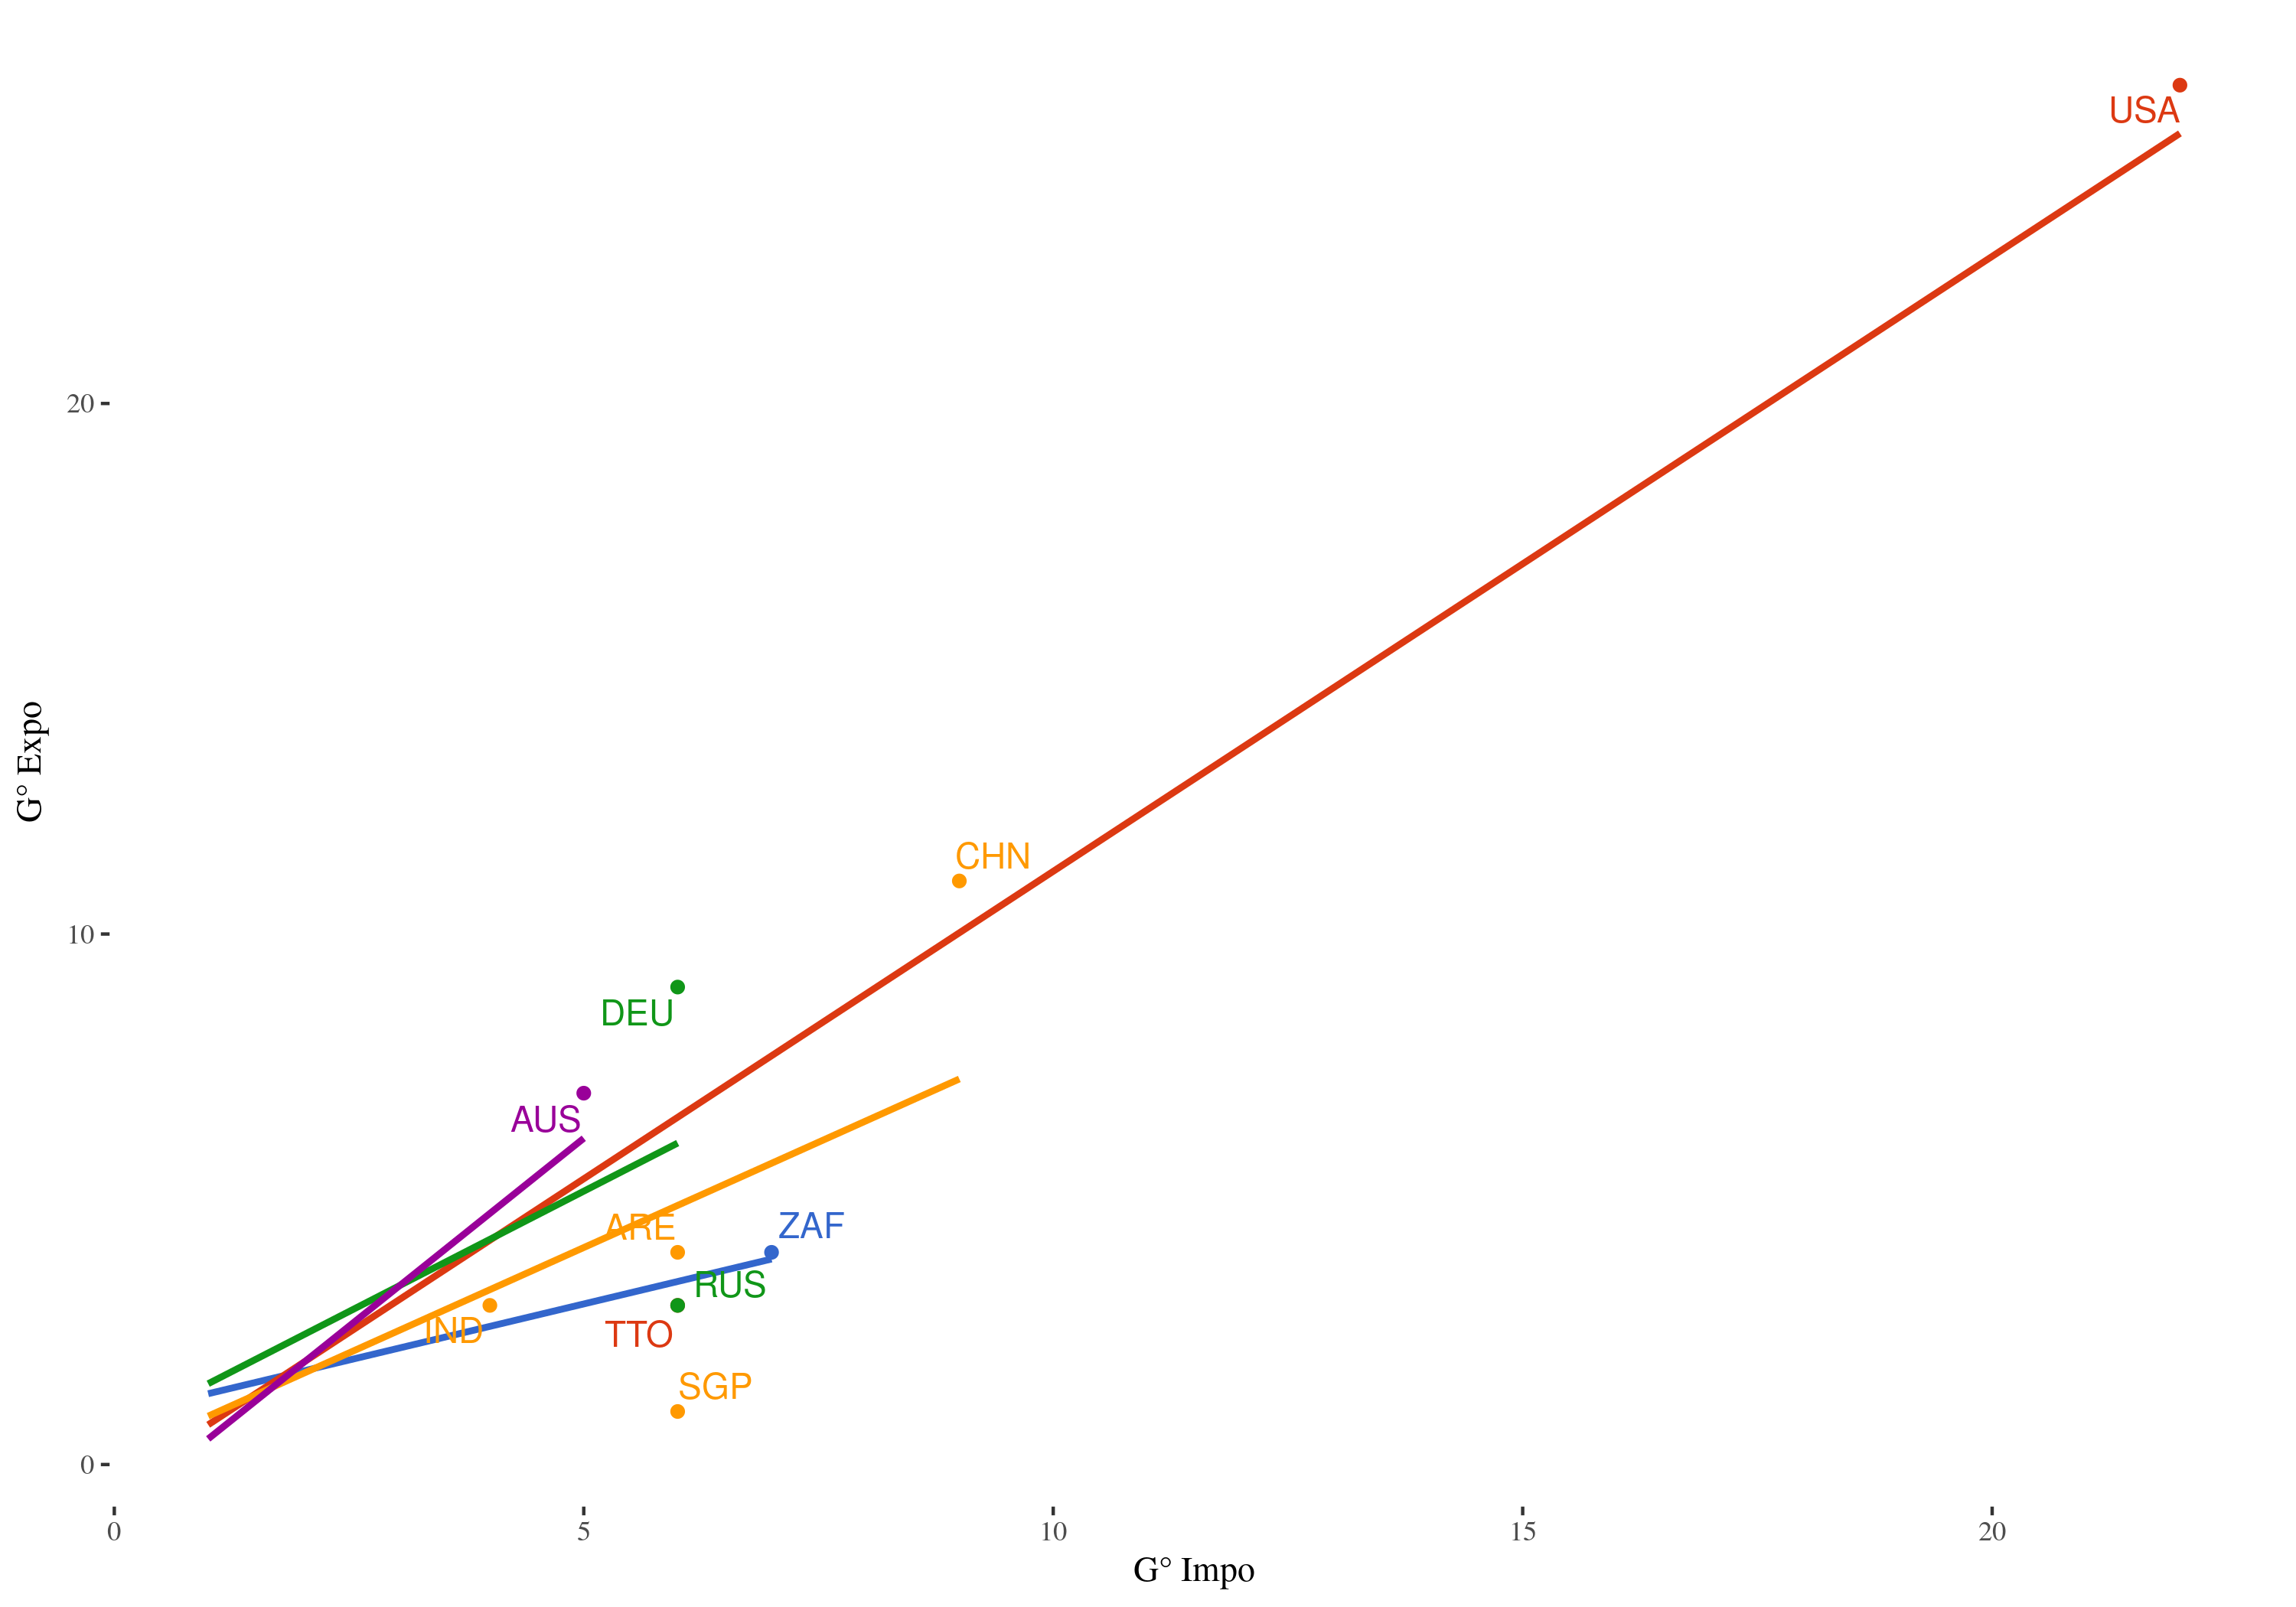
\includegraphics[width=\linewidth]{corr_grados_2011_20_pcnt}
		\end{figure}
	\end{flushleft}
	
	
	\column{.45\textwidth} % Left column and width
	\begin{itemize}
		\item 20\% Threshold: Strong dependency network
		\item Considering this type of relations, USA has much more centrality.
		\item South Africa appears for the first time as a central node.
	\end{itemize}
		\end{columns}
	\end{frame}
	
			
	%	\begin{onlyenv}<1-3>
	%	%	\begin{flushright}
	%	\begin{figure}
	%			\includegraphics<1>[scale=0.35]{corr_grados_2011_1_pcnt}
	%			\includegraphics<2>[scale=0.35]{corr_grados_2011_10_pcnt}
	%			\includegraphics<3>[scale=0.35]{corr_grados_2011_20_pcnt}
	%			\caption{\only<1>{1\% Threshold: Weak dependency network}
	%					 \only<2>{10\% Threshold}
	%				 	 \only<3>{20\% Threshold: Strong dependency network}}
	%	\end{figure}%	\end{flushright}
	%	\end{onlyenv}
	%	
	%	\end{frame}
	
	
	
	
	
	
	
		%------------------------------------------------
		\begin{frame}
		\frametitle{China-USA 1950-2000 \& 1997-2011}
		
	
		
		\begin{columns}[c] % The "c" option specifies centered vertical alignment while the "t" option is used for top vertical alignment
			
			\column{.45\textwidth} % Right column and width
				\begin{figure}
					\includegraphics<1->[scale=0.25]{1950_2000_impo_densidad_USA_CHN_grado}
				\end{figure}
			
			
			\column{.5\textwidth} % Left column and width
				\small{We can see evolution in time of the degree centrality distribution, and the place of China and USA in that kernel.} \par
			Degree.Threshold 1\%. Imports
			\begin{flushleft}
				\begin{figure}
					\includegraphics<2->[scale=0.35]{impo_densidad_USAvsCHN_grado_x_yr}
				\end{figure}
			\end{flushleft}
			
		\end{columns}
		\end{frame}
		
		\begin{frame}
		\frametitle{New International Division of labour -I}
		\framesubtitle{Global measures}
		\begin{columns}[t] % The "c" option specifies centered vertical alignment while the "t" option is used for top vertical alignment
			
			
				\column{.45\textwidth} % Right column and width
			\begin{figure}
				\vspace*{-1cm}
				\includegraphics<1->[scale=0.37]{1950_2000_coef_clustering_x_yr}
				\only<1->{Clustering coefficient}
				\only<1->{ \par \small{The network reduce it's regionalisms}}
			\end{figure}
			
			
			\column{.45\textwidth} % Left column and width
			\begin{flushleft}
				\begin{figure}
					\vspace*{-1cm}
					\includegraphics<2->[scale=0.4]{1950_2000_correlacion_x_yr}
					\only<2->{Correlation}
					\only<2->{ \par \small{Trade connections grows between central and non-central countries}}
				\end{figure}
			\end{flushleft}
		\end{columns}
		\end{frame}
		
		\begin{frame}
		\frametitle{New International Division of labour -II}
		\framesubtitle{Countries evolution}
		\begin{columns}[c] % The "c" option specifies centered vertical alignment while the "t" option is used for top vertical alignment
			
			
			\column{.35\textwidth} % Right column and width
			\begin{flushleft}
			\begin{figure}
				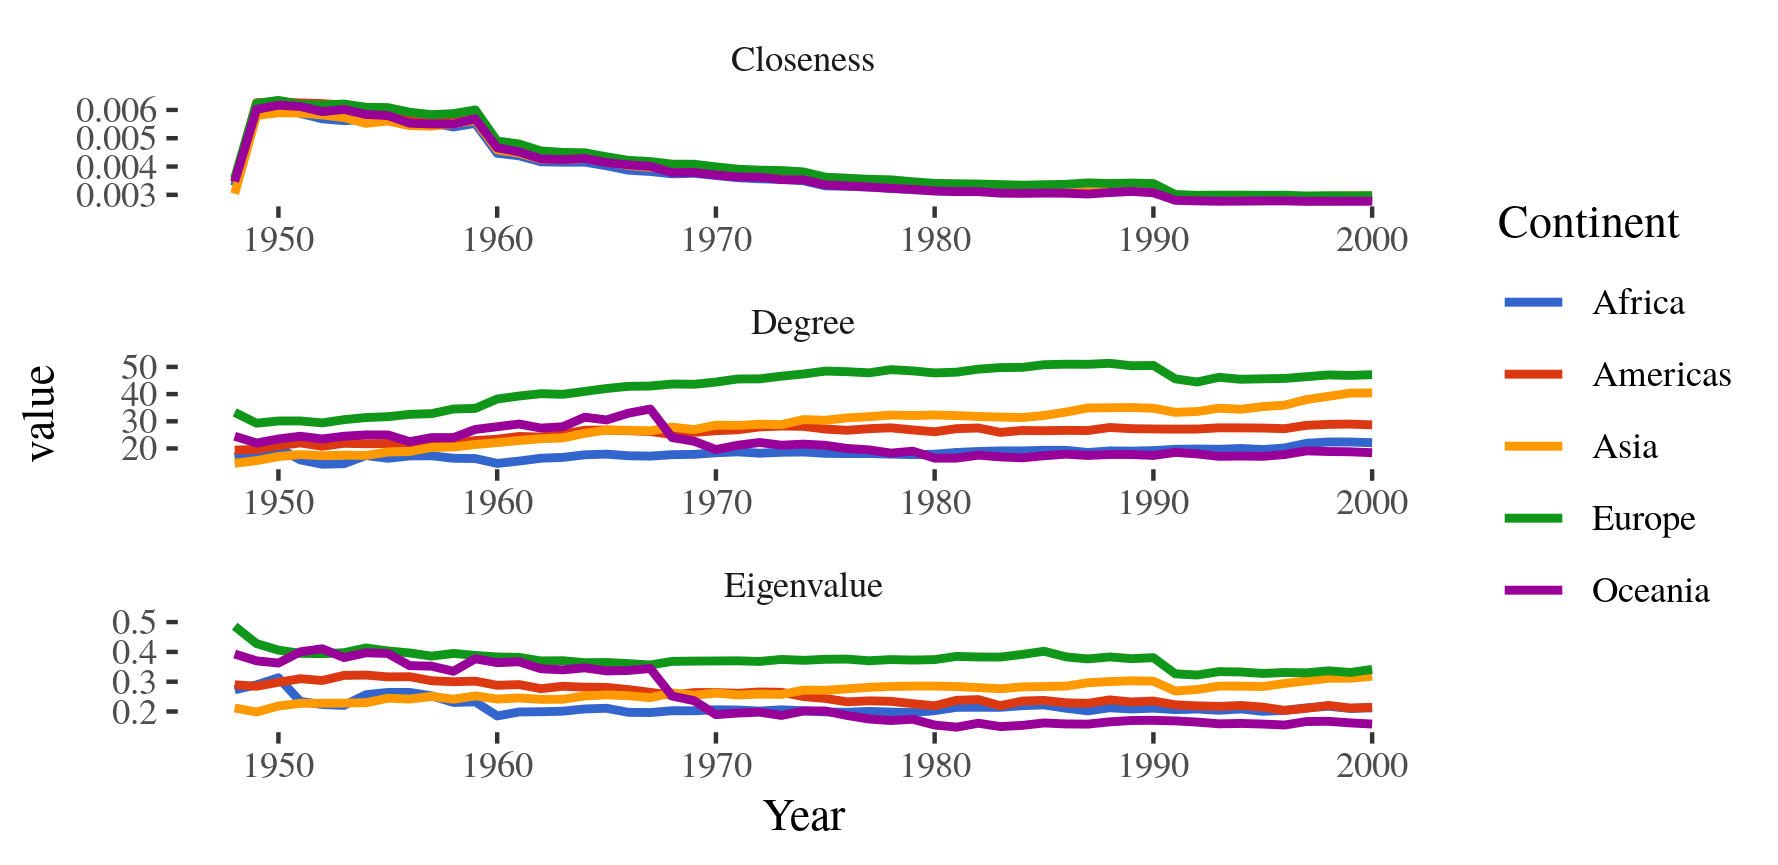
\includegraphics[width=2\linewidth]{1950_2000_continent_all_presentation}
			\end{figure}
			\end{flushleft}
			
			\column{.25\textwidth} % Left column and width\\
			
			
			\column{.45\textwidth} % Left column and width
			\begin{itemize}
				\item<1-> Closeness is a robust measure of the graph
				\item<2-> Asia goes from de last place to the second in Eigenvalue and Degree centrality
				\item<3-> Oceania goes from de second place to the last in Eigenvalue and Degree centrality
			\end{itemize}
		
		\end{columns}
		\end{frame}
		
		
		\begin{frame}
		\frametitle{New International Division of labour -III}
		\framesubtitle{Asia's role}
		\begin{columns}[c] % The "c" option specifies centered vertical alignment while the "t" option is used for top vertical alignment
			
			
			\column{.4\textwidth} % Right column and width
			\begin{flushleft}
				\begin{figure}
					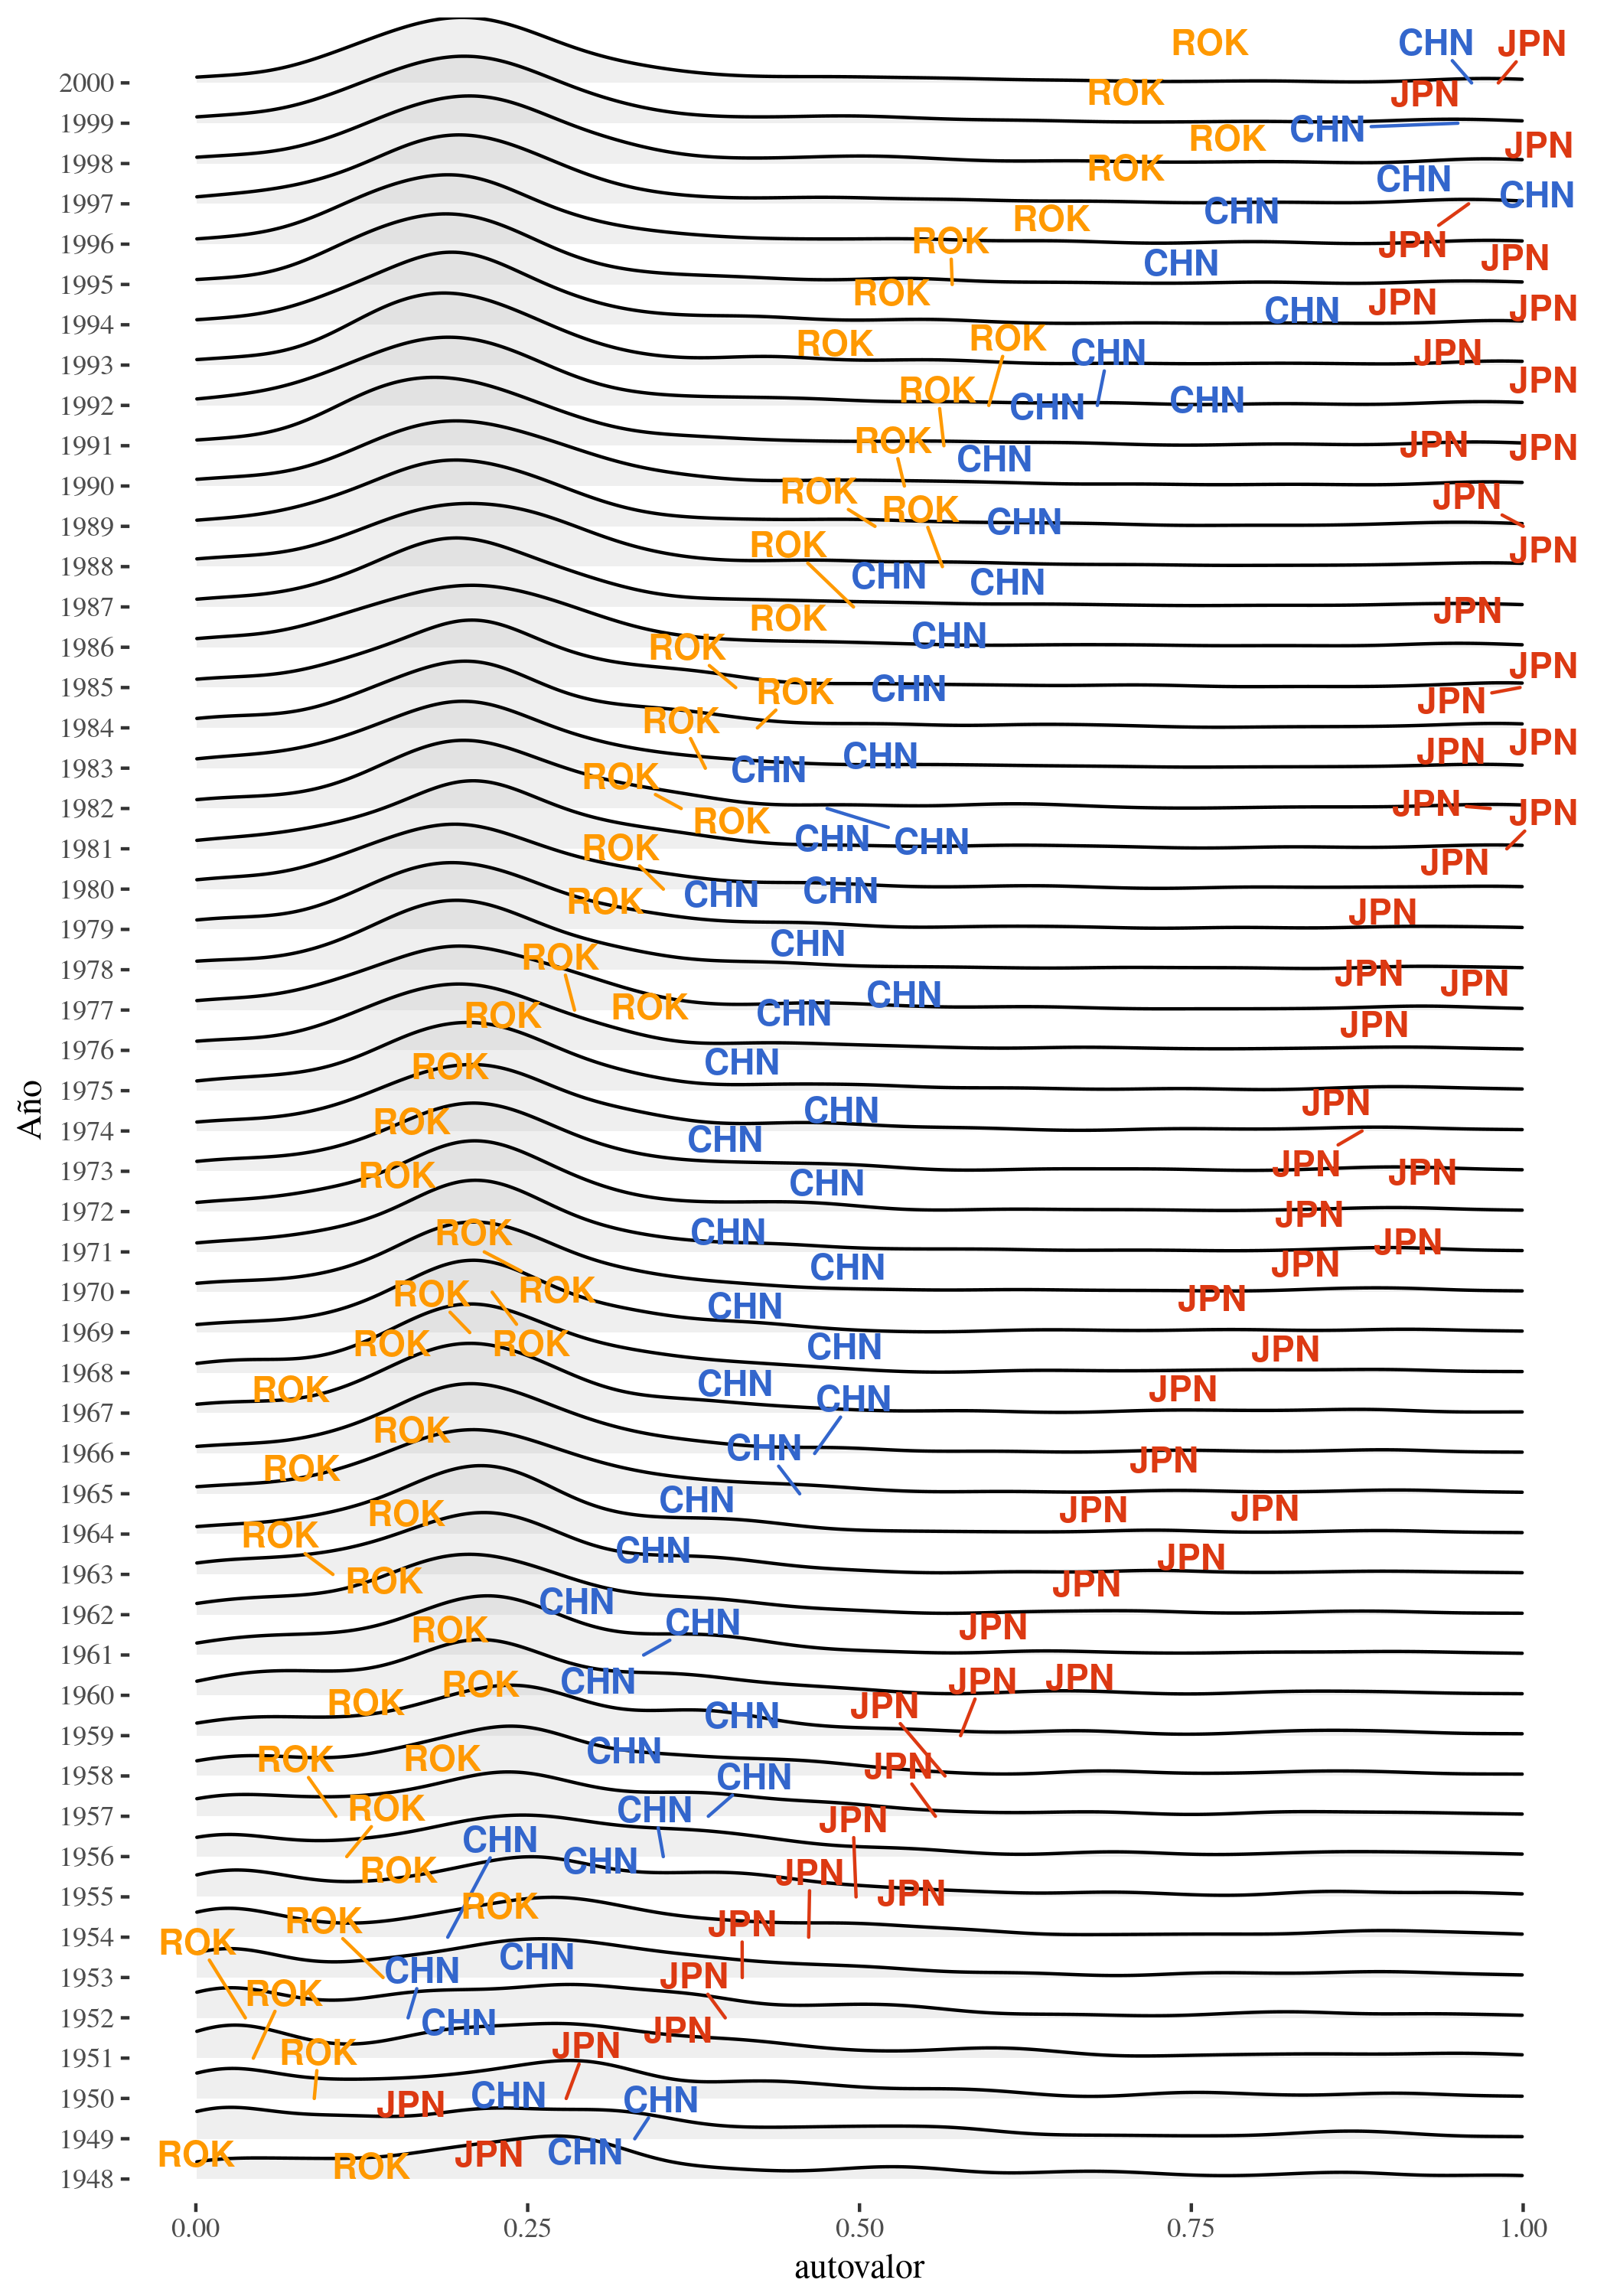
\includegraphics[width=\linewidth]{1950_2000_impo_densidad_CHN_JPN_ROK_atvlr}
					\only<1->{\small{Eigenvalue}}
				\end{figure}
			\end{flushleft}
			
			
			\column{.45\textwidth} % Left column and width
			\begin{itemize}
				\item<1-> Japan makes the same path to centrality, several years earlier
				\item<2-> South Korea also scales centrality positions in the graph, although starting from the back
			\end{itemize}
			
		\end{columns}
		\end{frame}
		
		\begin{frame}
		\frametitle{New International Division of labour -IV}
		\framesubtitle{Latin America}
		\begin{columns}[c] % The "c" option specifies centered vertical alignment while the "t" option is used for top vertical alignment
			
			
			\column{.45\textwidth} % Right column and width
			\begin{flushleft}
				\begin{figure}
					\includegraphics<1->[width=.9\linewidth]{1950_2000_impo_densidad_ARG_BRA_MEX_grado}
					\only<1->{\small{Degree}}
				\end{figure}
			\end{flushleft}
	
			\column{.45\textwidth} % Left column and width
	\begin{itemize}
		\item<1-> From the 80's, Brazil increases its commercial links with the rest of the world.
		\item<2-> Argentina and Mexico maintain their relative position in the period
	\end{itemize}
	
		
	\end{columns}
	\end{frame}
	
	\begin{frame}
	\frametitle{New International Division of labour -IV}
	\framesubtitle{Latin America}
	\begin{columns}[c] % The "c" option specifies centered vertical 		
			
			\column{.45\textwidth} % Left column and width
			\begin{flushleft}
			\begin{figure}
				\includegraphics<1->[width=.9\linewidth]{1950_2000_impo_densidad_ARG_BRA_MEX_atvlrpnd}
				\small{Weighted Eigenvalue}
			\end{figure}
		\end{flushleft}
			
			\column{.45\textwidth} % Left column and width
	\begin{itemize}
		\item<1-> If we see the Weighted Eigenvalue centrality, which consider the centrality of the countries partners, Mexico grows strongly from the 90's 
		\item<2-> This may be due to its relationship with the USA
	\end{itemize}
	
		\end{columns}
		\end{frame}
		
		\begin{frame}
		\frametitle{Conclusions}
		\begin{itemize}
			\item Network analysis have a great potential to describe Word Trade.
			\item We find that Europe and the United States play a more important role as consumers than as producers
			\item We also find that Asia, and China in particular, has a more central role in the world market in the last 60 years.
			\item Code: \url{www.github.com/DiegoKoz/grafo_comercio_agregado}
		\end{itemize}
		\end{frame}
	
		
		\begin{frame}
		\Huge{\centerline{The End}}
		\end{frame}
		
		%----------------------------------------------------------------------------------------
		
		\end{document}